\section{ALGORITHMS}  \normalfont

\subsection{Interactive Constrained MAP-Elites}
\label{sec:icmap-elites}

The~\acrfull{icmape}~\cite{alvarez2019empowering,Alvarez2020-ICMAPE} is the main algorithm developed in this thesis, which focuses on adapting the Constrained~\acrshort{mape} to be used in an~\acrshort{micc} system allowing designers to interact with it, and change non-intuitive aspects of~\acrshort{mape}. The main novel characteristics of~\acrshort{icmape} are:
% to be interacted by the designer. 

\begin{itemize}
    % \item Adapting~\acrshort{mape} to be used to co-design levels by proposing suggestions in an~\acrshort{micc} system.
    \item \acrshort{mape} adapted to be used in a~\acrshort{micc} system to collaborate and interact with the designer.
    \item Use of~\acrshort{mape} to create dungeons and adventure levels.
    \item Continuously adapting the fitness landscape and search space based on the designer's creation, which in turn, makes~\acrshort{mape} continuously adapting to a changing space.
    \item Customizable behavioral feature dimensions as part of the designer's ability to interact with the system. By changing the feature dimensions, pressure is imposed in the algorithm to adapt the search as the behavior dimensions are no longer the same (i.e., the niches changed).
\end{itemize}

In terms of the~\acrshort{ea} components, our implementation of~\acrshort{icmape} in~\acrshort{edd} uses direct encoding similar to the one depicted in figure~\ref{fig:directENCOD}, selection is through competition of individuals in each cell population, and selected individuals are applied crossover and mutation. Finally, the replacement strategy is elitist; if any offspring is better than individuals in their cell, these are replaced. 

Moreover, there are three ways designers can interact with~\acrshort{icmape}: 1) By editing their design, which automatically updates and adapt the fitness function. 2) By changing behavior feature dimensions and the size of cells, which is reflected in the algorithm's search space. And 3) By locking areas of their design to be preserved in the evolutionary run, which limits the building blocks~\acrshort{icmape} has to apply variation operators to, but preserves the designer's structures. This last interaction was developed earlier than~\acrshort{icmape} but is still available for the designer, is documented in~\cite{Alvarez2018a}, and presented in section~\ref{sec:desInteraction}.

\begin{algorithm}
%\algsetup{linenosize=\tiny}
\footnotesize
\caption{Interactive Constrained MAP-Elites}\label{alg:ICMAPE}
\begin{algorithmic}[1]
\Procedure{IC MAP-Elites($\protect[\{d_1,v_1\},...,\{d_n,v_n\}]$)}{}
\State $target \gets curEditRoom$ \Comment{Always in background}
\State createCells$(\protect[\{d_1,v_1\},...,\{d_n,v_n\}])$
\For{$i \gets 1$ to $PopSize$} %\Comment{$PopSize \gets 1000$}
     \State add mutate$(target)$ to $population$
\EndFor
\State CheckAndAssignToCell$(population)$ 
\While {true} \Comment{start continouous evo}
    \For{$generation \gets 1$ to $publishGen$}
        \If {$\textit{dimensionsChanged}$}
            \State $previousPop \gets cells_{pop}$
            \State createCells$(newDimensions)$
            \State checkAndAssignToCell$(previousPop)$ 
        \EndIf
        \MRepeat{ \text{[for feasible \& infeasible pop.]}}
            \For{$i \gets 1$ to $ParentIteration$}
                \State $curCell \gets \text{rndCell}(cells)$
                \State add tournament$(curCell)$ to $parent$
            \EndFor
            \State $offspring \gets  \text{crossover}(Parent)$
            \State checkAndAssignToCell$(offspring)$
        \EndRepeat
        \State sortAndTrim$(cells)$
    \EndFor
    \State broadcastElites() \Comment{render elites}
    \State $pop' \gets cells_{population}$
    \State add mutate$(cells_{pop})$ to $pop'$
    \State add $target$ to $pop'$
    \State checkAndAssignToCell $(pop')$
    \State sortAndTrim$(cells)$
\EndWhile
\EndProcedure
\Procedure{createCells(dimensions)}{}
    \ForEach{$dim \in dimensions $}
        \State add newCell$(dim_d, dim_v)$ to $cells$
    \EndFor
\EndProcedure
\Procedure{$\protect \text{check\&AssignToCell}(curPopulation)$}{}
    \ForEach{$individual \in curPopulation $}
        \State $individual_f \gets evaluate(individual)$ 
        \State $individual_d \gets dim(individual)$
        \State add $individual$ to $cell_{pop}(individual_d)$
    \EndFor
\EndProcedure
\end{algorithmic}
\end{algorithm}

In terms of execution,~\acrshort{icmape} is very similar to the vanilla~\acrshort{mape} and Constrained~\acrshort{mape} with three main differences: 1) The evolutionary run never ends and continuously update and adapts the fitness function based on the designer's current design, and through this, populations within cells might change their order, putting new pressure in individuals. 2) After $n$ amount of generations, the designer is presented a collection of suggestions in the same~\acrshort{mape} grid used in the search. When this happens, all individuals in all cells are selected, cloned, and minimally mutated to promote diversity. 3) At any moment, the designer might decide to replace their design with a suggested one, which in turn drastically change the algorithm, since rather than adapting the fitness gradually, the change might directly make high-performing individuals low-performing. However, one of the benefits of~\acrshort{mape} is it's fast convergence; thus, the algorithm adapts fast to the changes. And 4) the designer can change the feature dimensions (a pair at a time) and the amounts of cells per dimension to create bigger or smaller niches. Through this, the designer is effectively reshaping the behavior characteristics where encountered individuals in the search space will be retained, thus changing non-intuitive parameters in intuitive ways. The algorithm is depicted in listing~\ref{alg:ICMAPE}, and some examples of the~\acrshort{mape} grid presented to the designer are shown in figure~\ref{fig:MAPEGrid1}.

\begin{figure}[!h]
    \centering
     \subfloat[]{%
       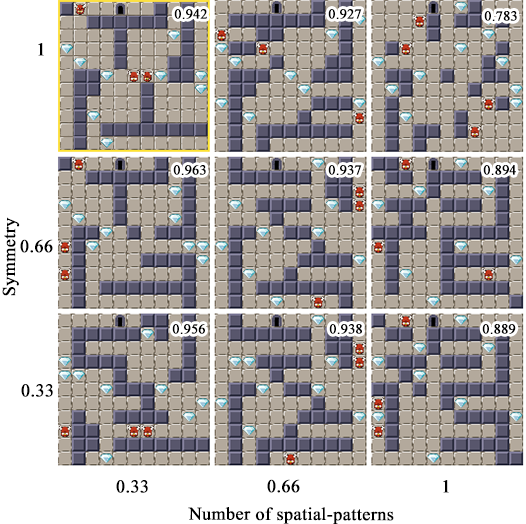
\includegraphics[width=0.49\textwidth]{figures/ICMAPE-figs/figure5.png}
     }
     \hfill
     \subfloat[]{%
       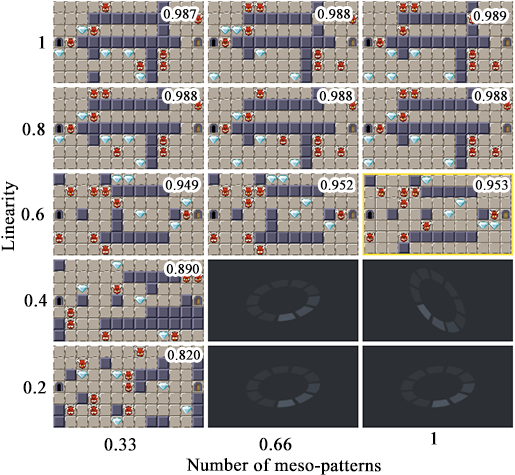
\includegraphics[width=0.49\textwidth]{figures/ICMAPE-figs/figure8.png}
     }
    
    \caption{Examples of suggestion grids presented to the designer as they design different rooms.}
    \label{fig:MAPEGrid1}
\end{figure}

As highlighted, behavioral feature dimensions are one of the main components of~\acrshort{mape} and all of its variations. They are context-dependent similar to fitness functions, with the caveat that they are only used to categorize and place individuals in cells. The features currently available in our implementation of~\acrshort{icmape} in~\acrshort{edd} are presented in table~\ref{table:mape-dimensions} along with a description of each dimension, and an example of each dimension and multiple cells in each dimension is shown in figure~\ref{fig:dimension-examples}. 
% While they are all related to the context of a dungeon and adventure games, there are two dimensions, \emph{similarity} and \emph{inner similarity}, which adapts dynamically to the current, i.e., at different time-steps, it will yield

\begin{table}[ht]
\centering
\caption{Developed game based features used as dimensions in the~\acrlong{icmape}}\label{table:mape-dimensions}
% \resizebox{\textwidth}
% \resizebox{\textwidth}
\begin{tabularx}{\textwidth}{|c|X|}
\hline
\rule{0pt}{12pt}
Feature&Definition\\ \hline
% \\[-6pt]
Similarity & Refers to the aesthetic (tile-by-tile) similarity between a room and the current designer's design.\\ \hline
Inner Similarity & Refers to the similarity of the sparsity and density of the different tile types of a room designer's current design.\\ \hline
Symmetry & Refers to the aesthetic symmetry of a room.\\ \hline
Leniency & Refers to how challenging rooms are; calculated based on the position of enemies and balance between enemies and treasures.\\ \hline
Linearity & Refers to the amount of paths connecting doors within a room; calculated based on how many spatial patterns are traversed.\\ \hline
\#Meso-Patterns & Refers to the number of meso-patterns that exist within a room, normalized by an estimated maximum number based on the room's size and the minimum chamber size.\\ \hline
\#Spatial-Patterns & Refers to the number of spatial-patterns that exist within a room, which can be chambers, corridor, turns, junctions, and intersections.\\ \hline
\end{tabularx}
\end{table}


Finally, Mouret and Clune discuss that a traditional single-objective approach could reach as good fitness in an individual for some of the tasks they experimented~\cite{Mouret2015}. Nevertheless, 1) this would only focus on obtaining one high-performing individual, 2) the search would focus in fewer places of the generative space, and as a consequence, and 3) the diversity of the generated individuals would be scarce. The nature of our mixed-initiative tool not only requires but promotes the identification of multiple solutions that would satisfy similar constraints. For instance, a linear room could be one with narrow corridors connecting doors or a simple open chamber containing all doors. Therefore, a rich, diverse, and high-performing set of levels to be suggested to the designer that could be generated in a short period, and that can adapt to changes over time is a key necessity for~\acrshort{edd}. 
% This motivated the development of~\acrshort{icmape} and is  and essential feature of~\acrshort{icmape}, the motivation for developing~\acrshort{icmape}.

\begin{figure}[!ht]
\centerline{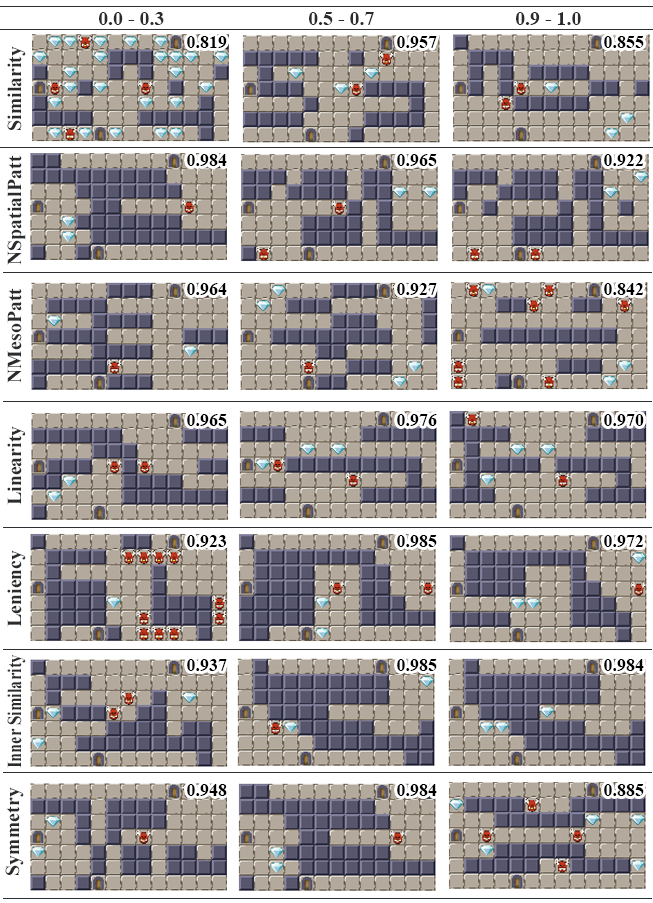
\includegraphics[width=0.7\textwidth]{figures/ICMAPE-figs/figure-all-dimensions-final.png}}
\caption{Example of Elites generated using IC MAP-Elites. Each row represents an independent run of the algorithm using the dimension specified to the left. Each column splits the dimension score into three intervals: 0.0-0.3 (low), 0.5-0.7 (medium), and 0.9-1.0 (high). Each cell displays (top-right) the fitness of the optimal individual in its related interval} \label{fig:dimension-examples}
\end{figure}

\subsection{Designer Preference}

To explore designer modeling and its benefits, the designer's preference model was proposed to drive the content generation in~\acrshort{icmape}~\cite{Alvarez2020-DesignerPreference}. In this work, the suggested~\acrshort{mape} grid is used to compose a dataset used as an estimator of the designer's preferences. The goal and motivation of modeling the designer's preferences were to use a surrogate model that could capture the designer's subjective evaluation and an objective evaluation from the fitness function. The model, the training, and the usage is depicted in figure~\ref{fig:desPrefModel}. 

\begin{figure}
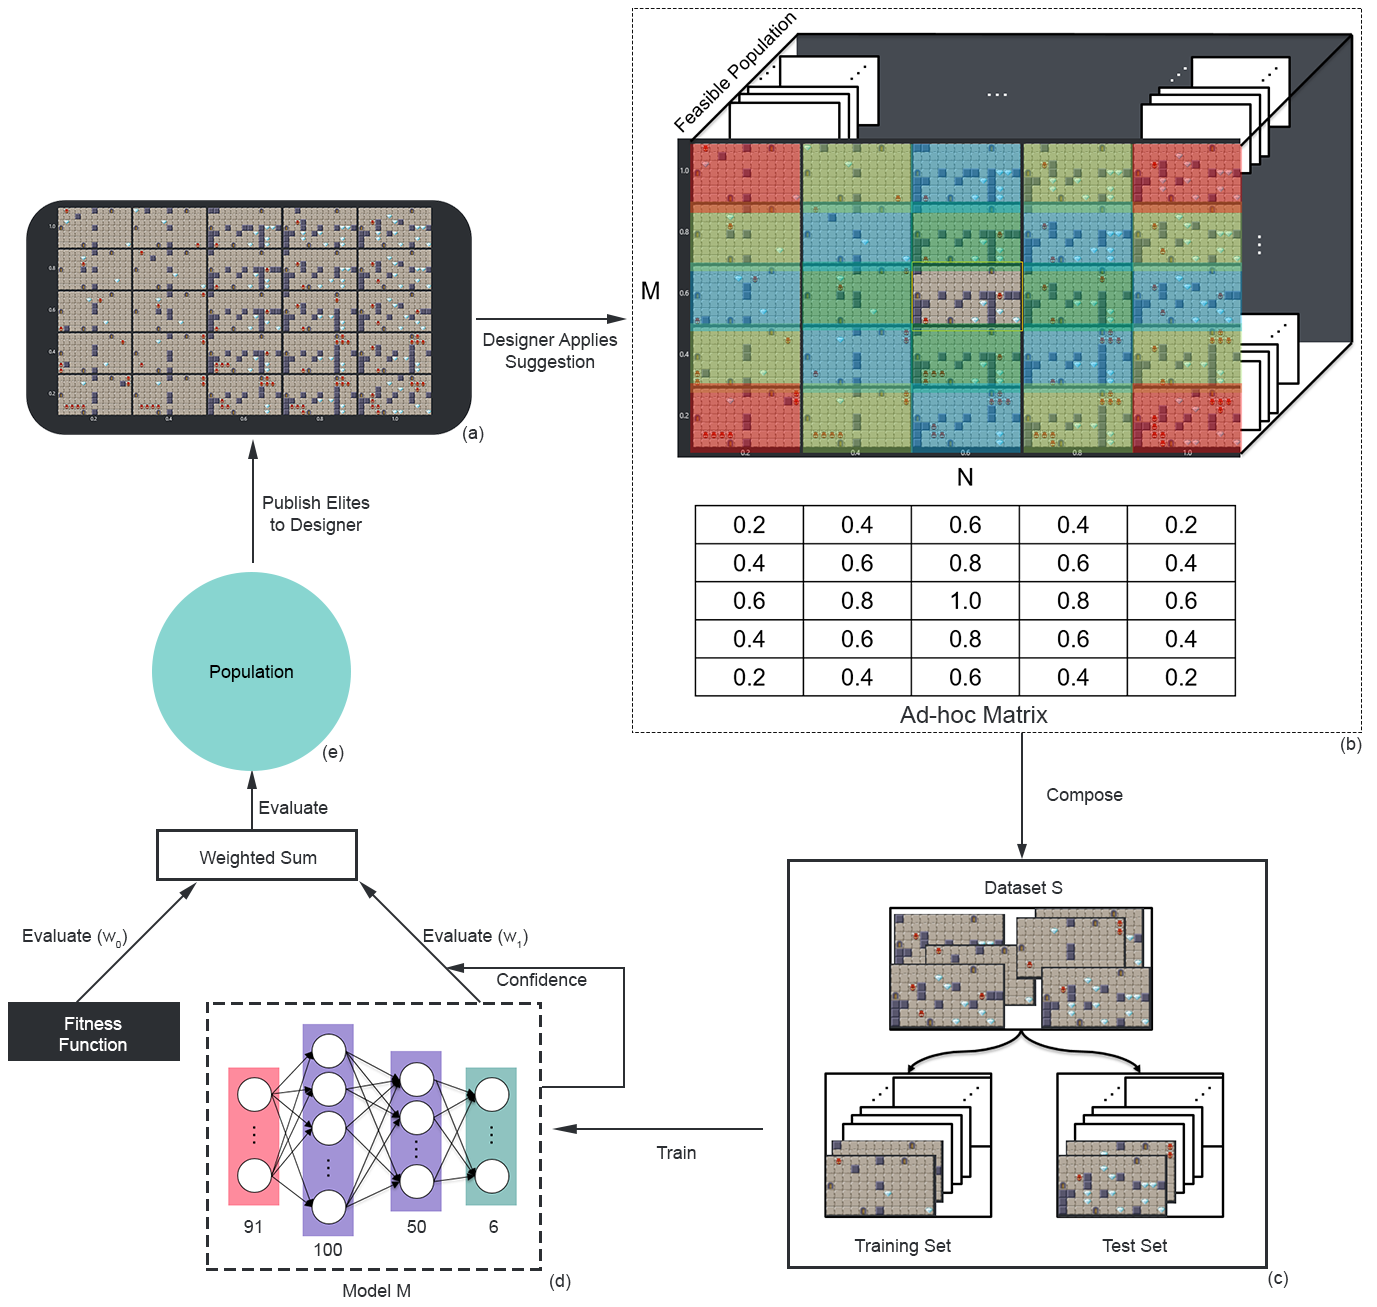
\includegraphics[width=\textwidth]{figures/DesPref-figs/desPrefModel.png}
\caption{Overview of the Designer Preference Model integrated into the fitness function of EDD. Elites are published and shown to the designer in a grid fashion (a). Once the designer chooses and applies one of the suggestions, an ad-hoc matrix is created based on the selected suggestion's position to estimate the preference of suggestions (b). The ad-hoc matrix is then applied to all the elites in the grid and the feasible populations within the EA cells to compose a general dataset $S$ with rooms labeled by the estimated preference. The composed dataset $S$ is then subdivided into a training set (90\%) and test set (10\%), both with the same label distribution (c). The dataset is used to train a model $M$, which is a relatively small neural network for 20 epochs (d). The model is then used to evaluate the population of the EA together with the current fitness function in a weighted sum. The weight of the model $M$ conditioned by the confidence of the network (e).} \label{fig:desPrefModel}
\end{figure}

Following a proactive learning approach~\cite{donmez2008proactive}, whenever the designer chooses some suggestion, the system trained a learning model $M$ (i.e., a neural network) with a new set of preferred content (dataset $S$) using the current suggested cells and their population. The result was an adapted model similar to the work by Liapis et al.~\cite{Liapis2012-adaptiveVisual}, which learned overtime the designer's preferences in relation to their choices. Once the model is trained, it is incorporated in the evolutionary loop to drive evolution by means of evaluating the content in a weighted sum with the fitness function. The model slowly fits towards the designer’s preference, and as it's predictions become more confident, the more weight $W_{1}$ it has in the final evaluation. Confidence is calculated based on the softmax layer's output, which can be interpreted as probabilities for each class. The evaluation resulted in the weights (Eq.~\ref{eq:weights}) and the final weighted sum (Eq.~\ref{eq:weightedSum}).

\begin{equation} \label{eq:weights}
\begin{split}
 w_{1}={}&\min(M_{conf} \cdot M_{TestAcc}, 0.5),\\
w_{0} ={}& 1.0 - w_{1}   
\end{split}
\end{equation}

\begin{equation} \label{eq:weightedSum}
weightedSum = (w_{0} \cdot objective) + (w_{1} \cdot predicted_{pref})
\end{equation}

We evaluated the model and its usability in a user study with fifteen game design students. While not significant as there was not enough data to demonstrate the advantage of the model, the results allowed the analysis of the system's challenges. These challenges were presented as three open areas for active research: \textit{Dataset}: the type and amount of data collected; \textit{Preference modality}: what represents preference in the design and creative process; and \textit{Dynamic-Dynamic System vs. Dynamic-Static System}: the competing properties of a dynamic learning environment, e.g., a designer that traverse the design space, with a dynamically adapting model, e.g., a learning model that tries to adapt as the designer traverse the design space, and it's trade-offs.

\subsection{Style Clustering and Designer Personas}

\begin{figure}
\centerline{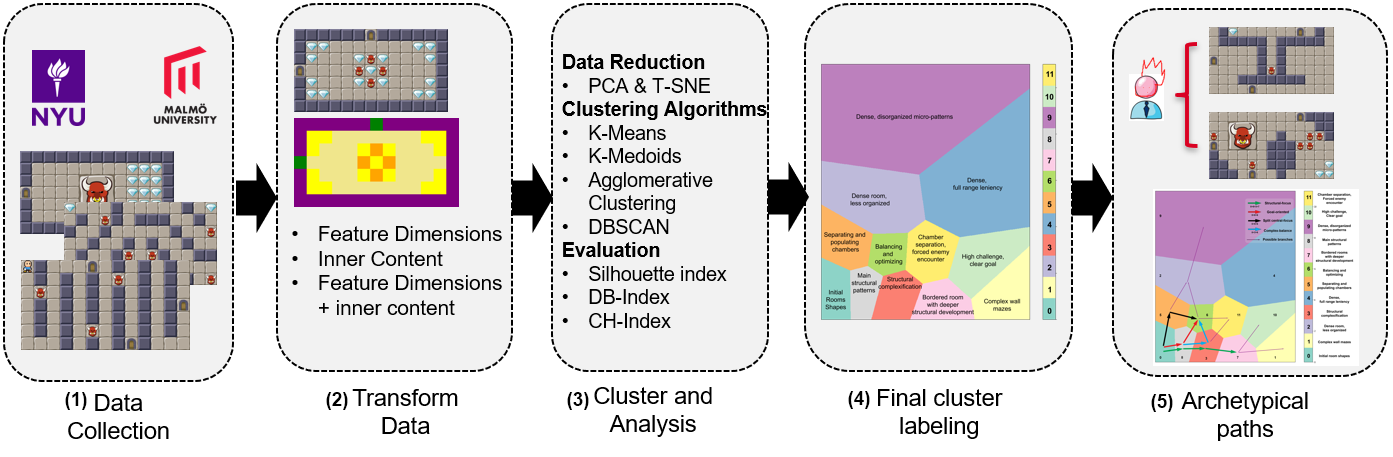
\includegraphics[width=\textwidth]{figures/DesPersonas-figs/process-steps.png}}
\caption{The stages of the design style clustering development: (1) Data was first collected through two user studies. (2) Then, using the design sequences, the data was processed into five different datasets, one using the room images, a second using the tiles information, and three using tabular information. (3) A data reduction technique was applied to different datasets, and then they were clustered and internally evaluated. (4) The clusters were formed, picked from the best-performing methods, and labeled based on the data points within each cluster. The clusters were evaluated by visualizing how a typical design session traverse the various clusters, and K-Means (K=12) was chosen as the final approach. (5) Finally, using this final approach, all the sequences were clustered, and archetypical paths were identified.
} \label{fig:clusteringApproach}
\end{figure}

To further explore designer modeling, an alternative approach was proposed by clustering designers' design styles~\cite{alvarez2020-designerpersonas}. The basic premise was that by identifying a set of styles that most designers follow when creating content, and model how the designer traverse such a style space, a model that captured the designer's intentions, goals, and style could be created. For instance, rooms for a game like the binding of Isaac~\cite{bindingISAAC} could be classified based on multiple characteristics such as the room's objectives regarding enemies and treasures, access to different areas, or hidden challenges and treasures. Moreover, different designers could reach the same room style through different paths, where the focus along the creation could vary. Some designers would focus on the room's topology before anything else, whereas others would focus first on the objectives a player must achieve. 

\begin{figure}[t]
\centerline{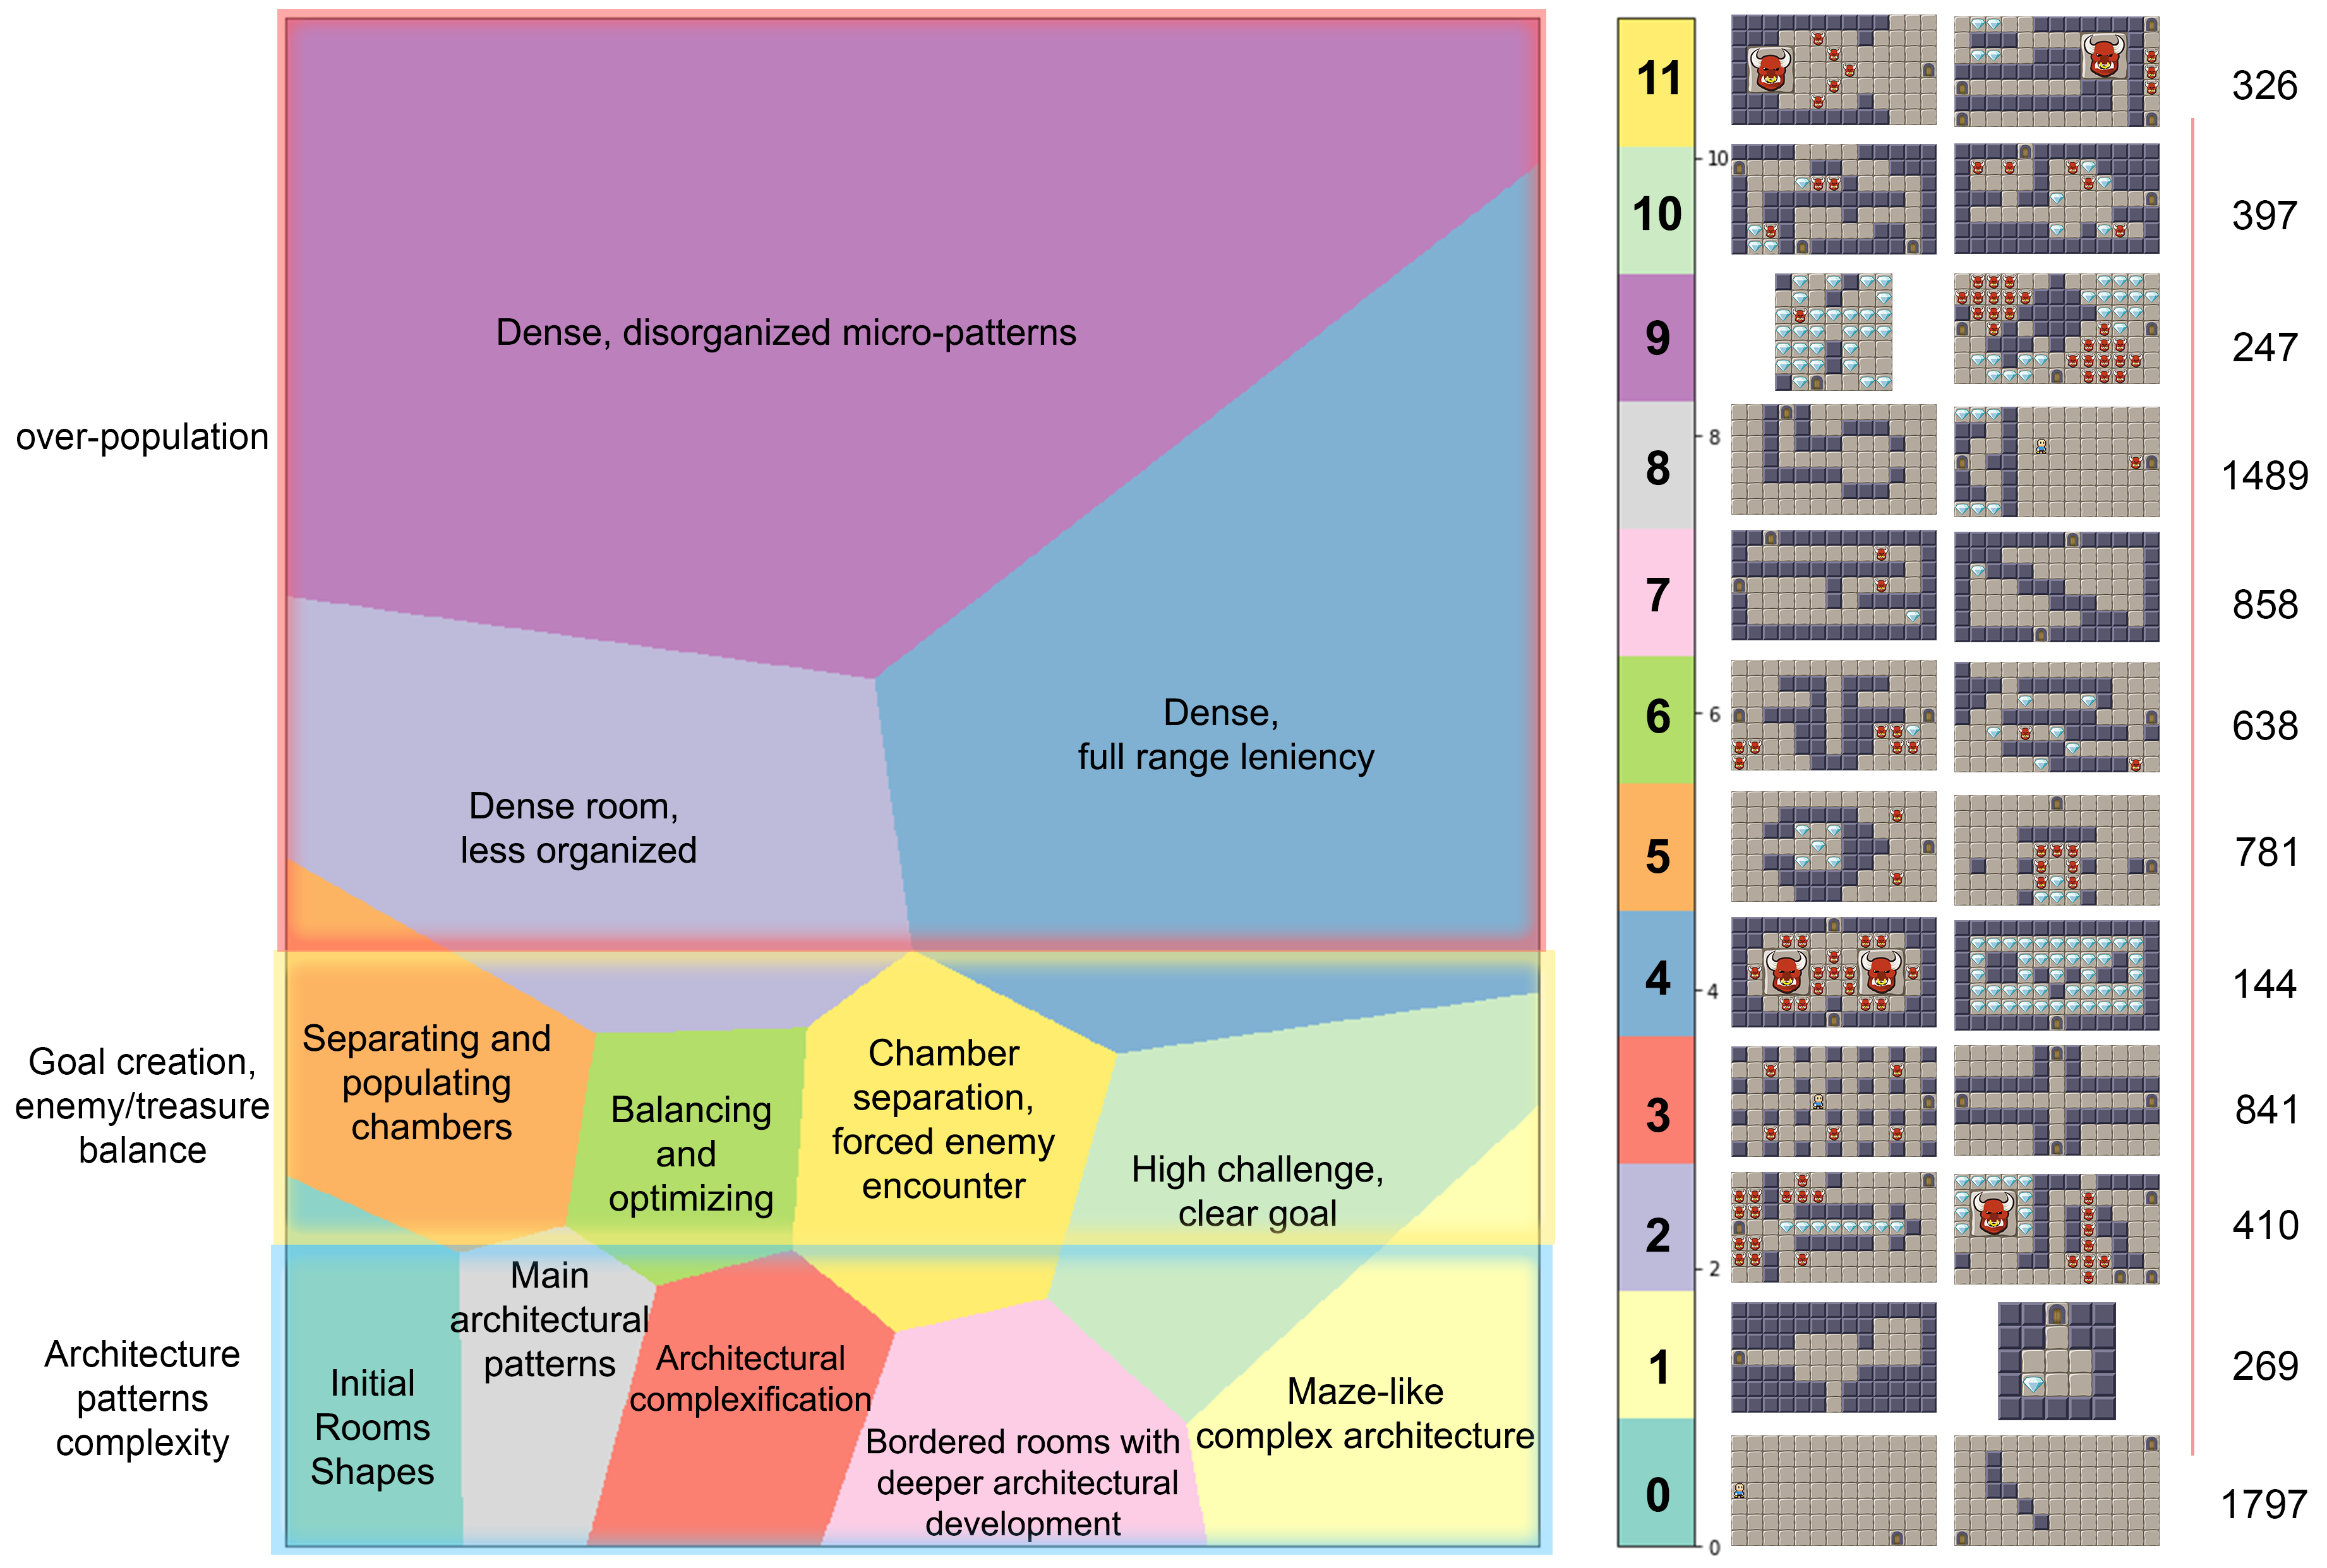
\includegraphics[width=\textwidth]{figures/DesPersonas-figs/final-cluster.png}}
\caption{Best resulting cluster set. K-Means (K=12), using the \textbf{Tiles} Dataset. While it scores slightly less in the internal indices that other setups, a qualitative analysis successfully gives us more granularity by subdividing the main bottom clusters to label and cluster designers' design process. Sample rooms belonging to each cluster are displayed on the right, next to the total number of rooms in the cluster.} \label{fig:all-clusters}
\end{figure}

With such as motivation and objective, it was compiled data of designers' designs and their creation process in the~\acrshort{edd} to create these models. The data was collected from two user studies, the one documented in the Designer's Preference Model previously described~\cite{Alvarez2020-DesignerPreference} with game design students, and another with practitioners and academic researchers within the computational intelligence in games area. The data was used to create five different datasets that were used in the experiment to analyze multiple variations and possibilities. The datasets were analyzed, experimented on, and compared to obtain the final clusters that effectively divided the design style space. The process is shown in figure~\ref{fig:clusteringApproach}. Figure \ref{fig:all-clusters} shows the final design style clusters with the setup that performed best among all the different experiments (K-Means (K=12), using the \textbf{Tiles} Dataset).

\begin{figure}[t!]
\centerline{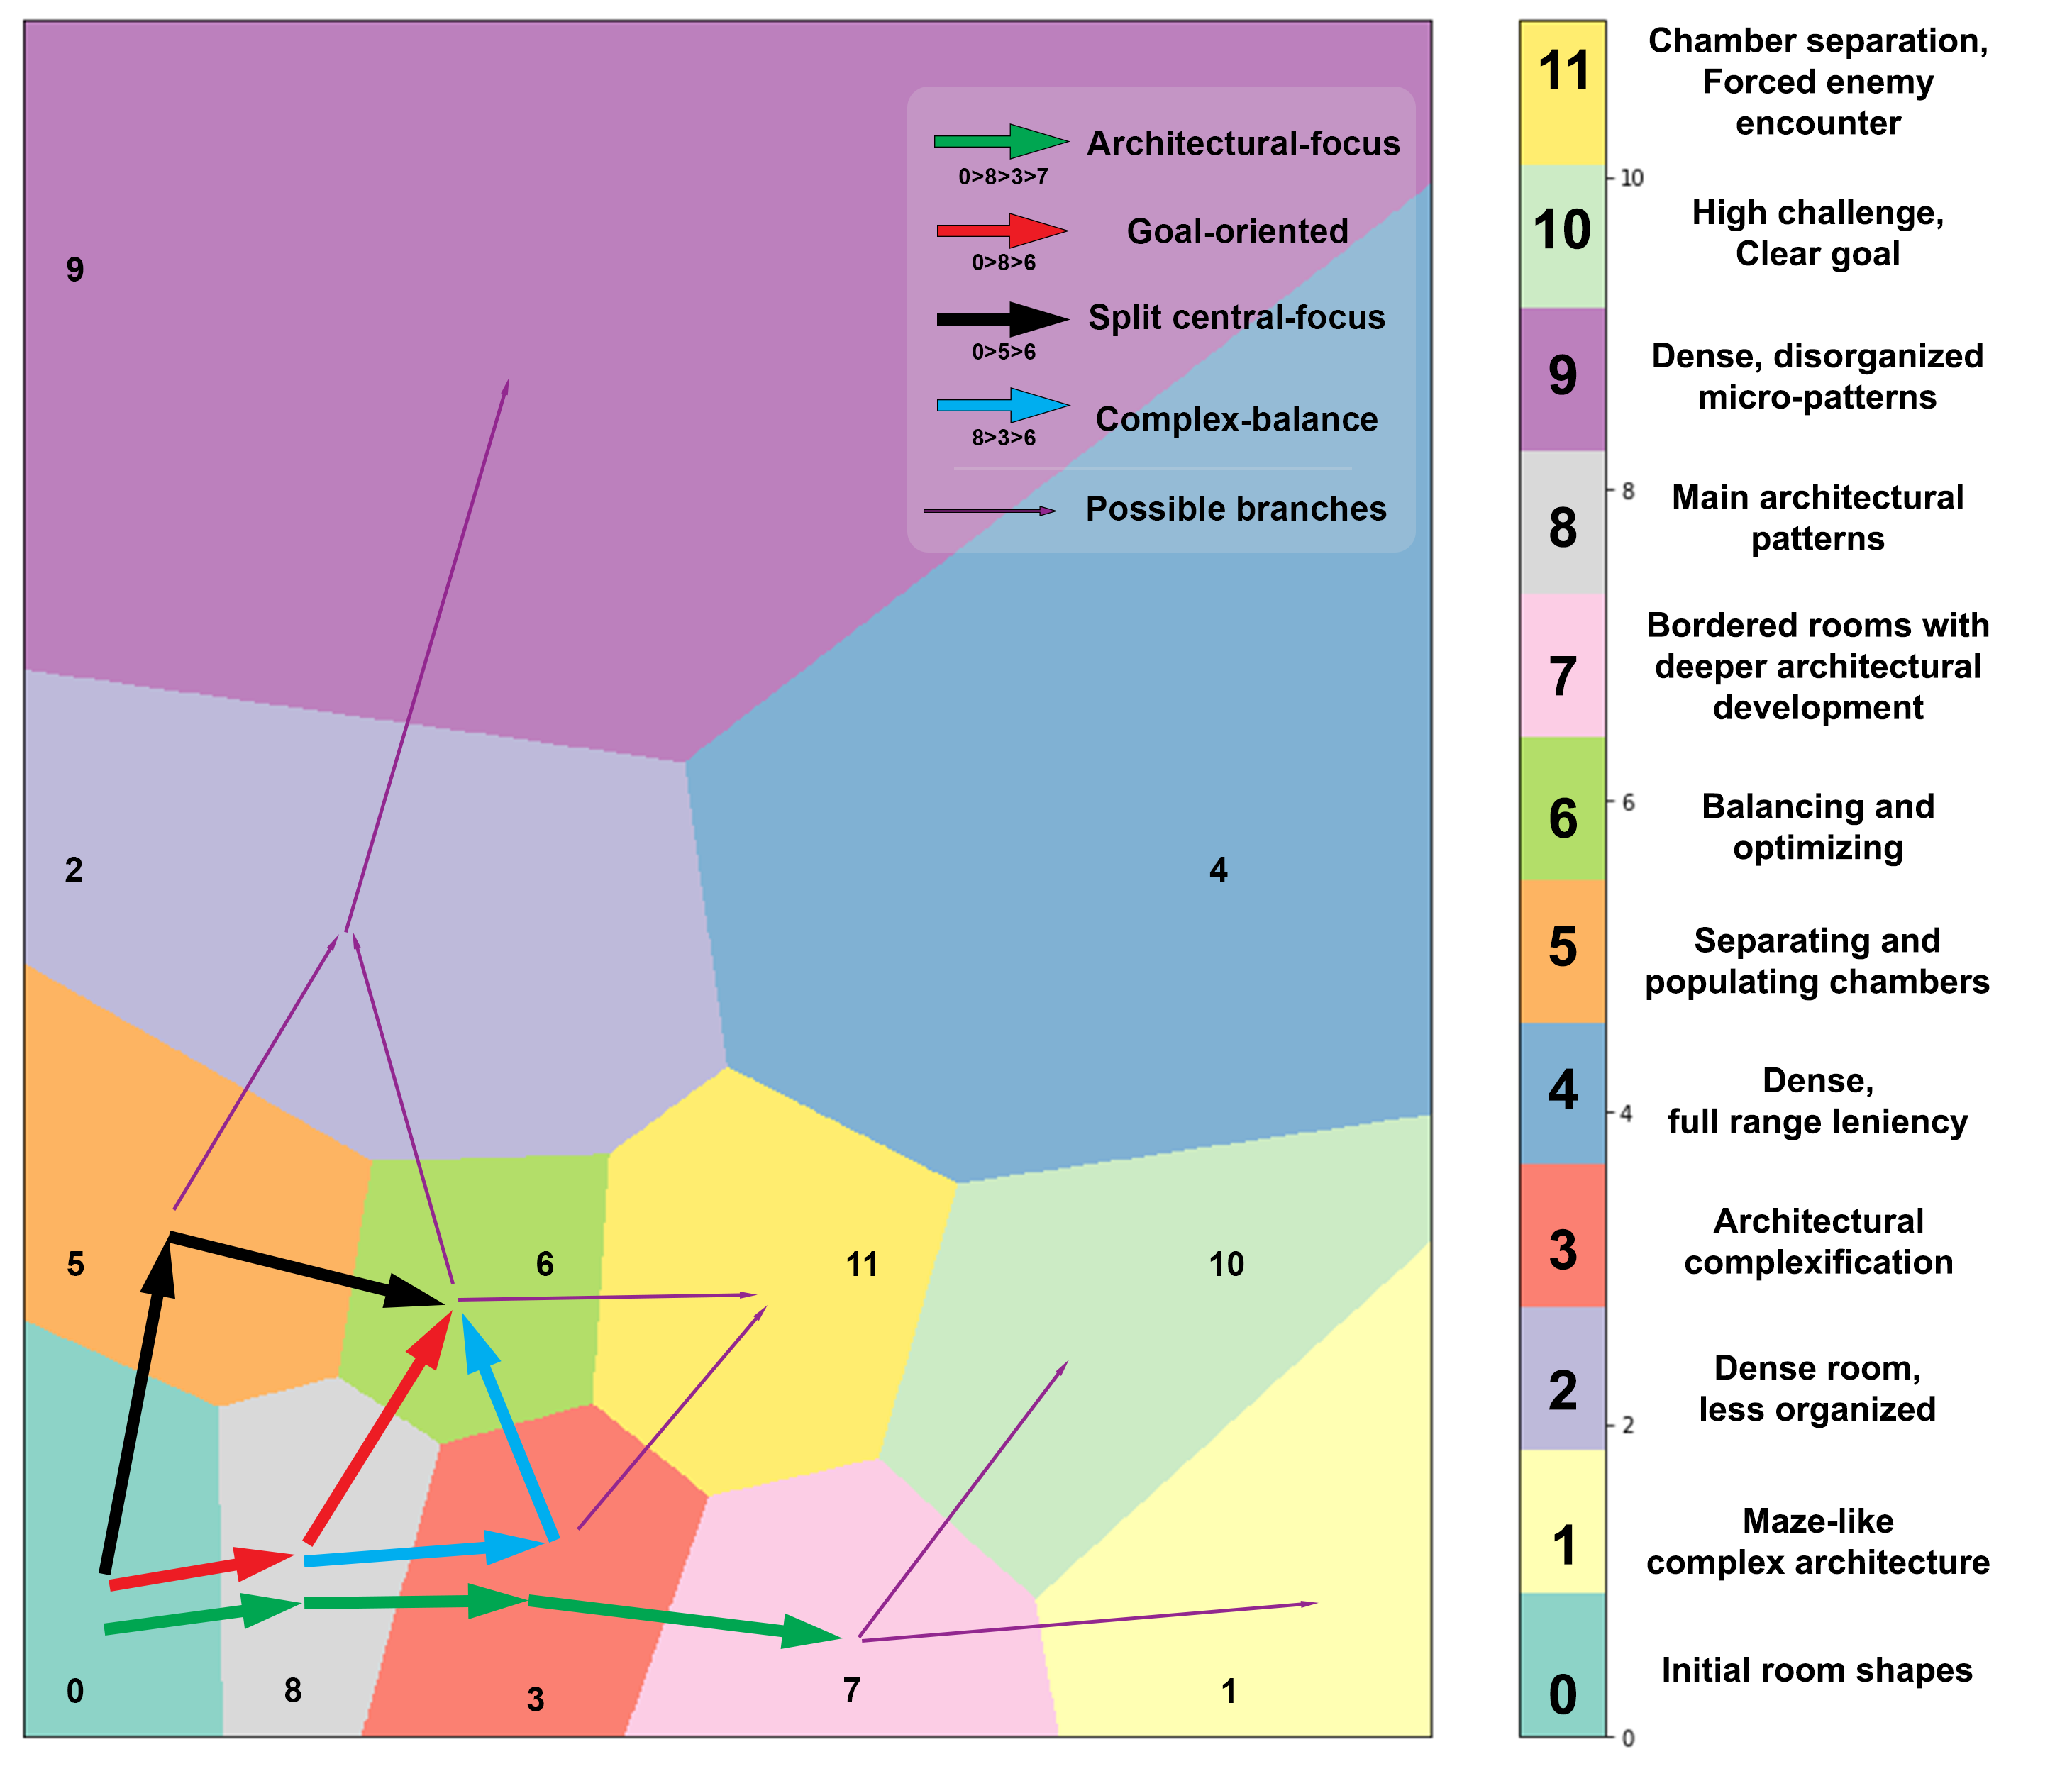
\includegraphics[width=\textwidth]{figures/DesPersonas-figs/resulting-paths-FINAL.png}}
\caption{Final and common designer trajectories. With thick arrows it is presented the archetypical paths, calculated using the frequencies of subsequences from $180$ diverse rooms. Each color represent a unique trajectory; with green the \textsc{Architectural-focus}, with red the \textsc{Goal-oriented}, with black the \textsc{Split central-focus}, and with blue the \textsc{Complex-balance}. Finally, thinner purple arrows extending from clusters traversed by the archetypical paths show the multiple possible branches that an archetypical path can deviate or extend to.} \label{fig:desPersonas}
\end{figure}

Moreover, with the design style cluster, we could then analyze the design process in function of the traversed clusters rather than evaluating each individual step. To do this, we analyzed the traversed clusters as unique trajectories. We gathered the common patterns from the trajectories by applying the Generalized Sequential Pattern (GSP) algorithm, which locates frequent subsequences in the analyzed trajectories. Through this, four \textit{designer personas} were identified. \textit{Designer personas} are defined as archetypical paths through style space that are commonly taken by designers when creating their content. In figure~\ref{fig:desPersonas} it is shown the identified \textit{designer personas}.
% , and figure~\ref{fig:desPersonasExamples} it is presented representative examples per each designer persona.

% \begin{figure}[t]
%     \centering
%      \subfloat[\textsc{Architectural-focus}\label{subfig-1:dummy}]{%
%       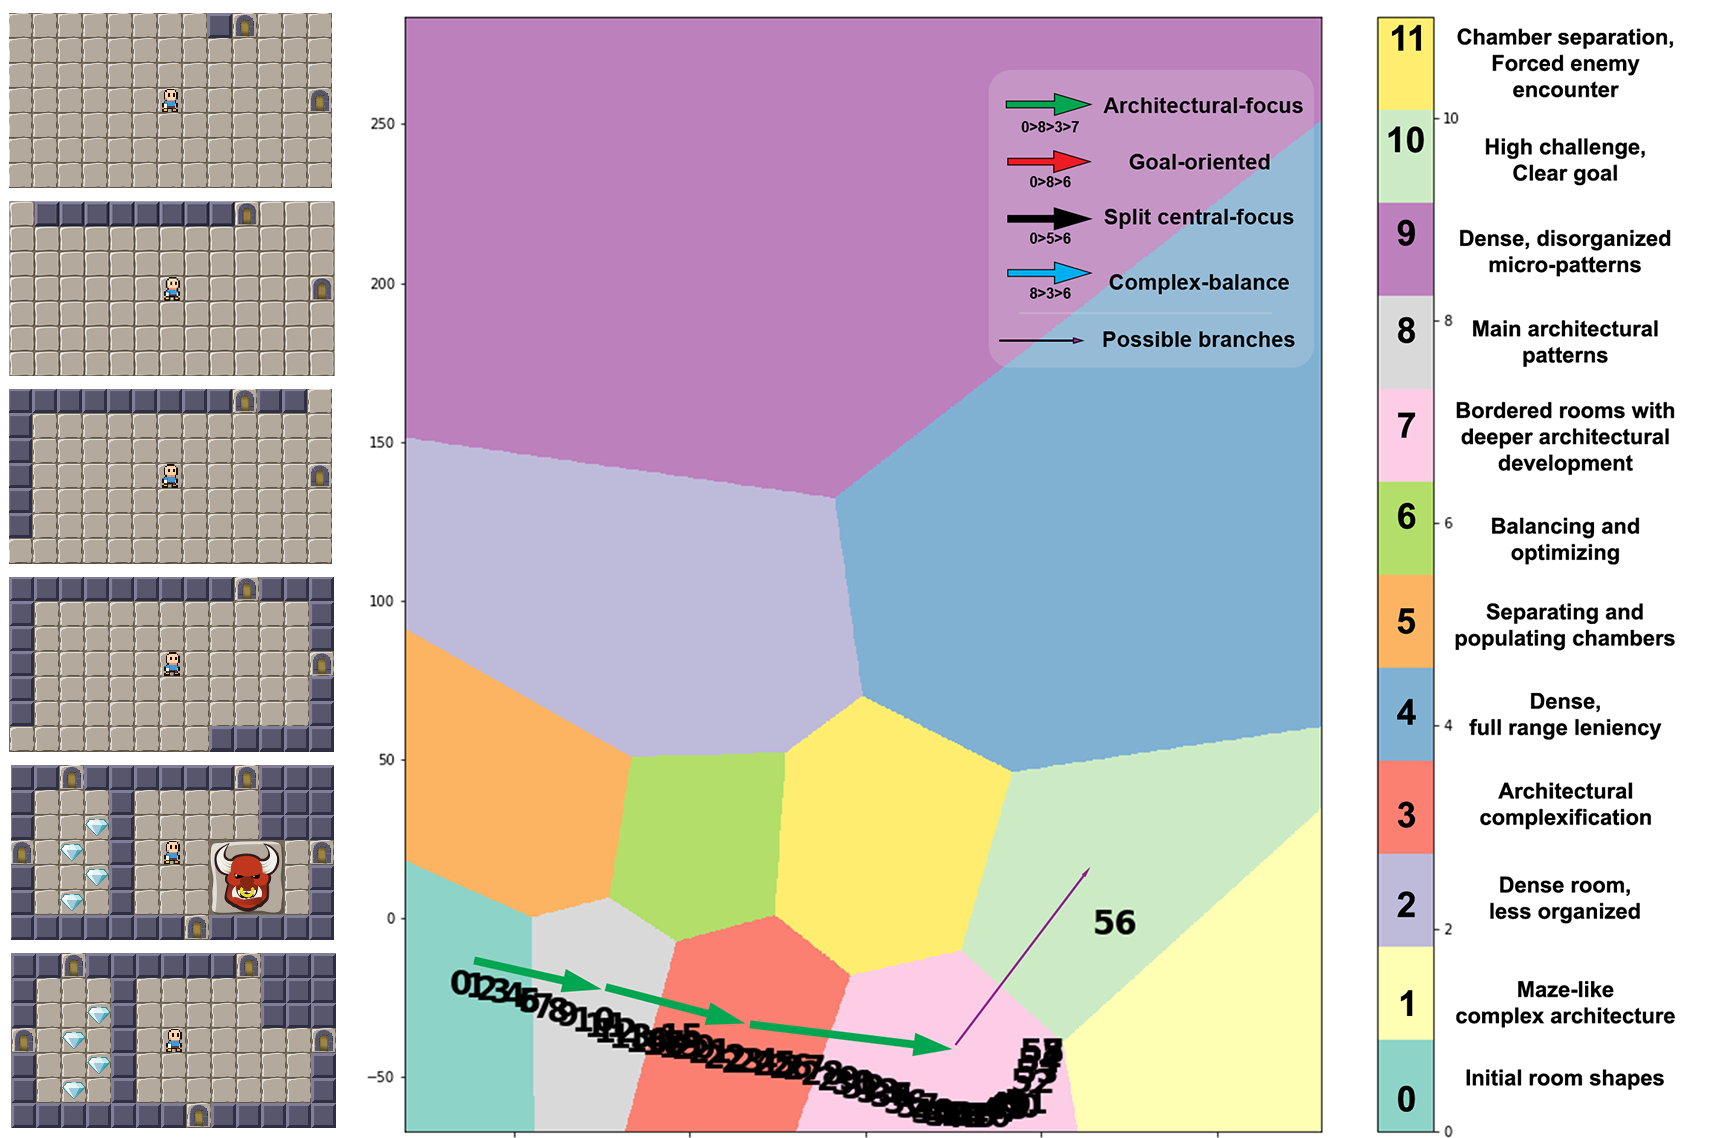
\includegraphics[width=0.6\textwidth]{figures/DesPersonas-figs/1.png}
%      }
%      \hfill
%      \subfloat[\textsc{Goal-oriented}\label{subfig-2:dummy}]{%
%       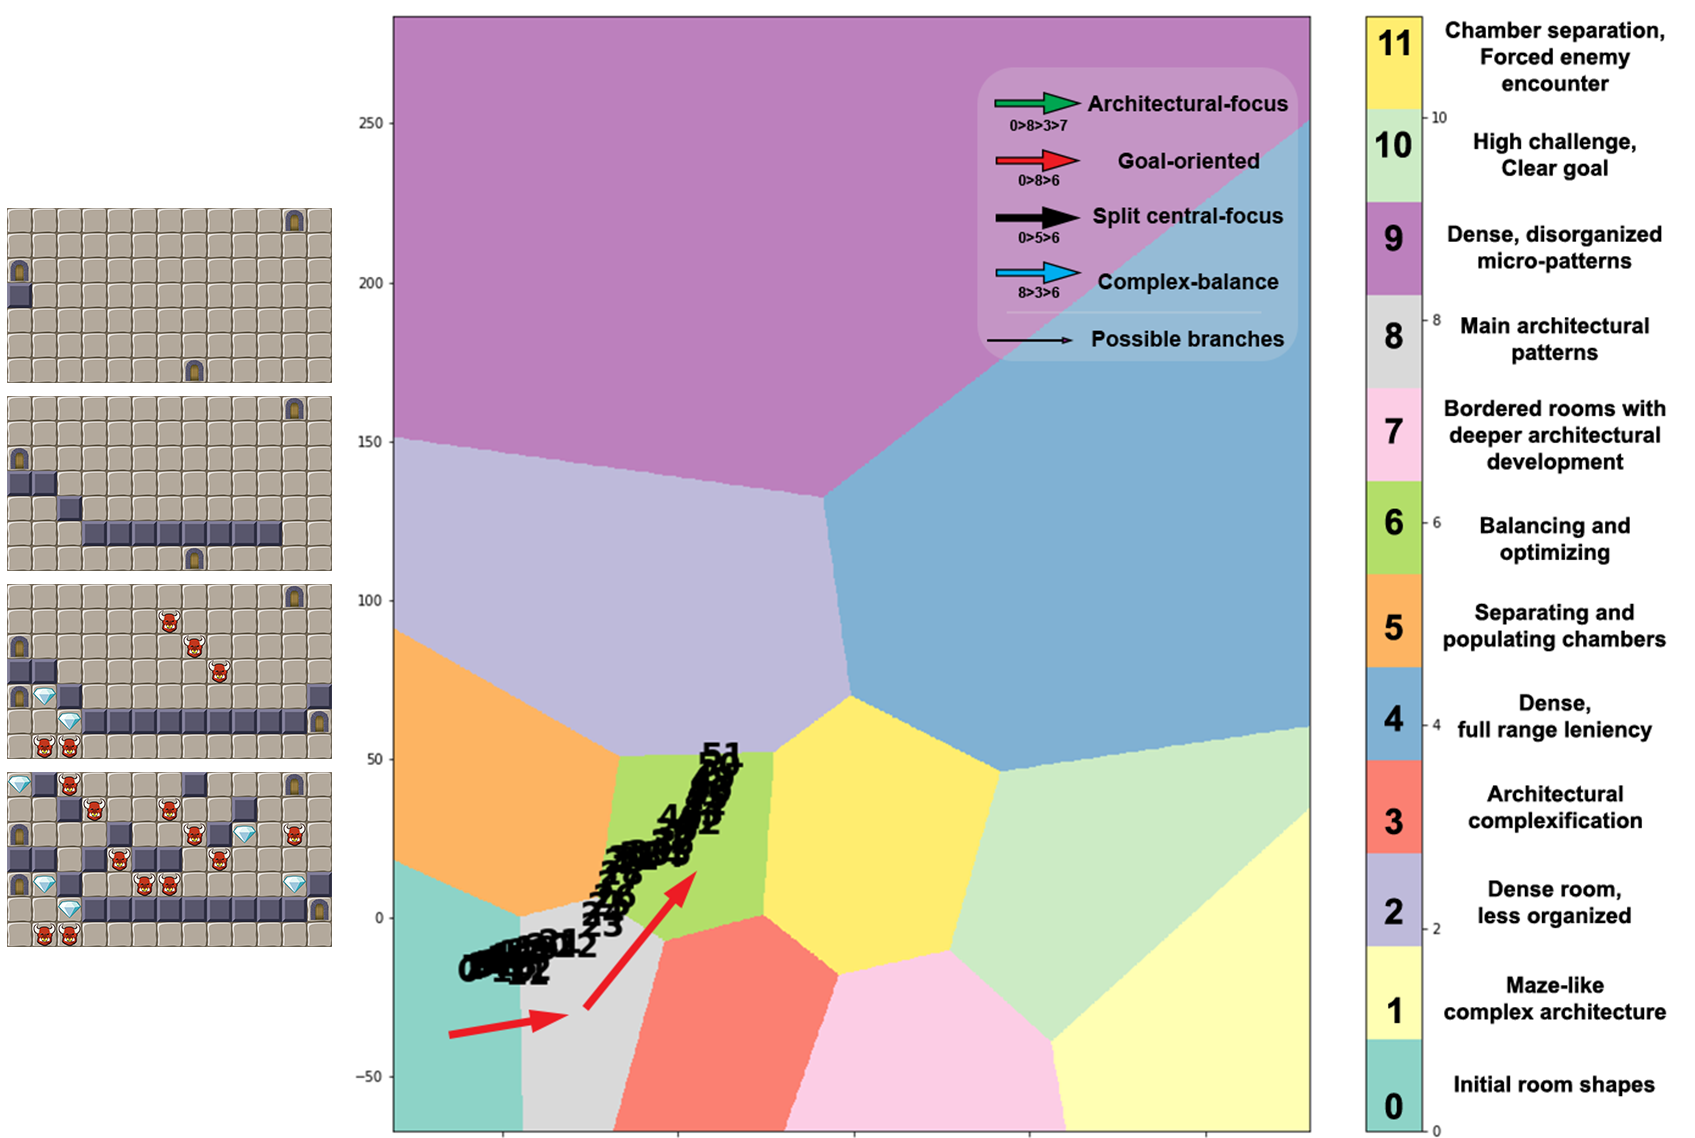
\includegraphics[width=0.45\textwidth]{figures/DesPersonas-figs/2.png}
%      }\hfill
%     %  \medskip
%      \subfloat[\textsc{Split central-focus}\label{subfig-3:dummy}]{%
%       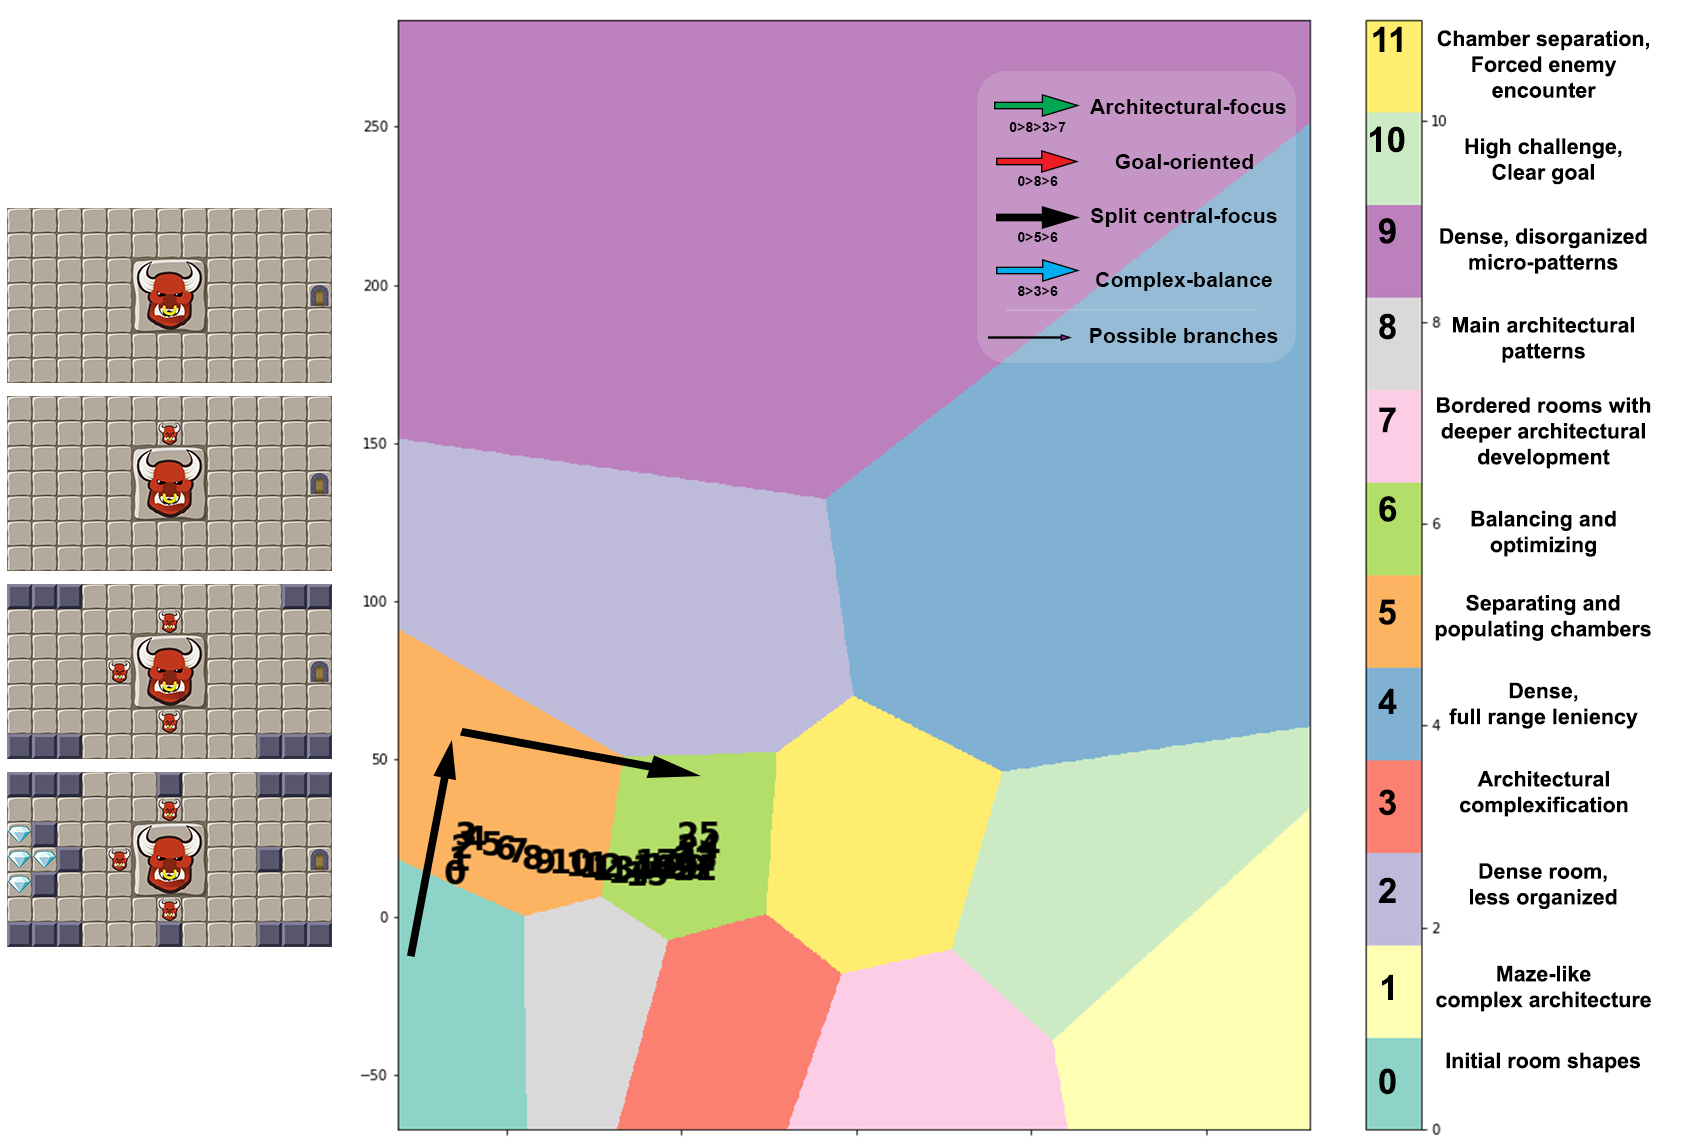
\includegraphics[width=0.45\textwidth]{figures/DesPersonas-figs/3.png}
%      }
%      \hfill
%      \subfloat[\textsc{Complex-balance}\label{subfig-4:dummy}]{%
%       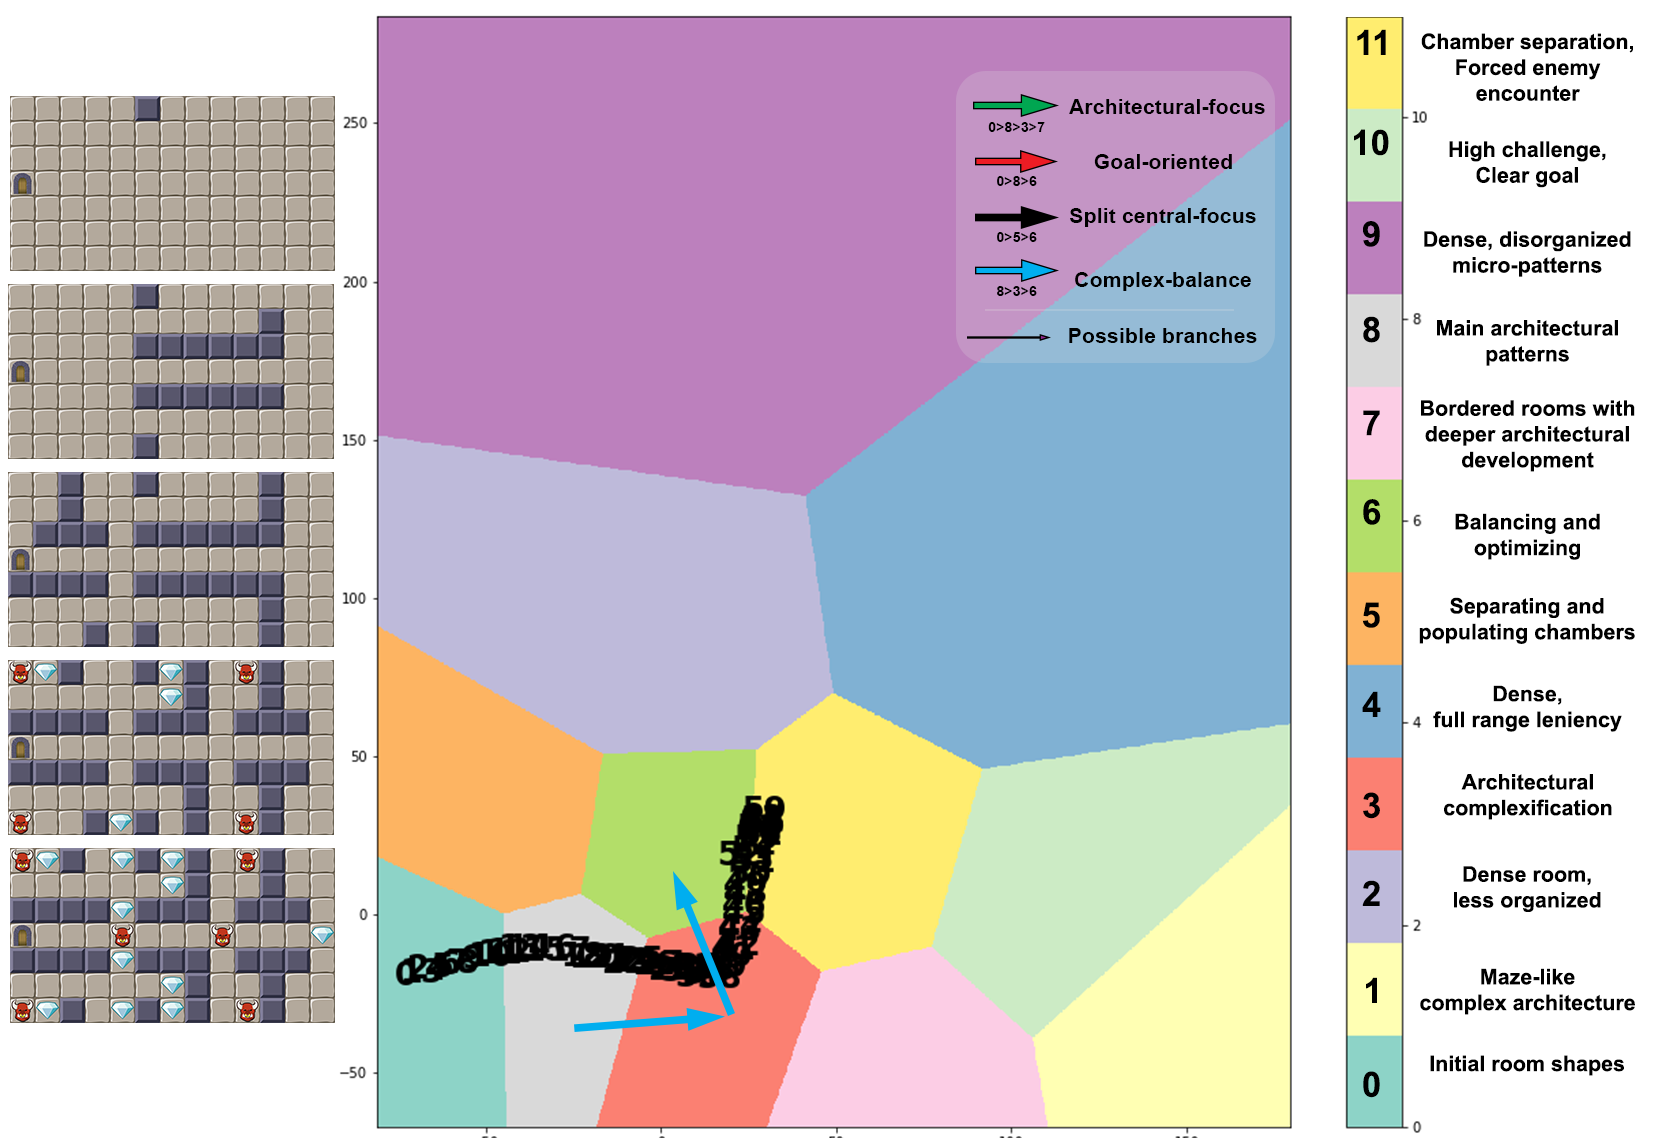
\includegraphics[width=0.6\textwidth]{figures/DesPersonas-figs/4.png}
%      }
    
%      \caption{Examples of each of the archetypical paths from one of the frequent sequences used to create the clusters. To the left of each subfigure, we present each key step in the trajectory i.e., when the design entered a new cluster. (a) presents the \textsc{Architectural-focus} archetypical path where the focus is firstly on creating the structural design of the rooms; the design process jumps back and forth suddenly to cluster 10 (one of the possible branches) due to the designer adding a boss and removing it immediately. (b) presents the \textsc{Goal-oriented} archetypical path where the design focus on a minimal structure complexity and mix between adding structural changes and enemies/treasures. (c) shows the \textsc{Split central-focus} archetypical path where, intentionally, the designer creates a center obstacle with a boss and build around it. Finally, (d) presents the \textsc{Complex-balance} archetypical path; the design focuses on building complex, uncommon structures first and then add some goal to it with enemies and treasures, taking advantage of the spaces.}
%     \label{fig:desPersonasExamples}
% \end{figure}
